\chapter{Background}
\label{cha:relatedwork}

In this section, the global system known as \emph{devices cloud} will be first detailed. Afterwards, the reader will be introduced to the different possible protocols and technologies that could be used. Finally, an overview of the different researches and studies that have been previously performed will be given.
 
\section{The Devices Cloud}
Integrating the requirements defined in the Introduction to a more detailed view of the global system, the Figure \ref{fig:design_complete} of the \emph{devices cloud} architecture . Of course, only the information relevant for this thesis is depicted.

\begin{figure}[!ht]
	\centering
	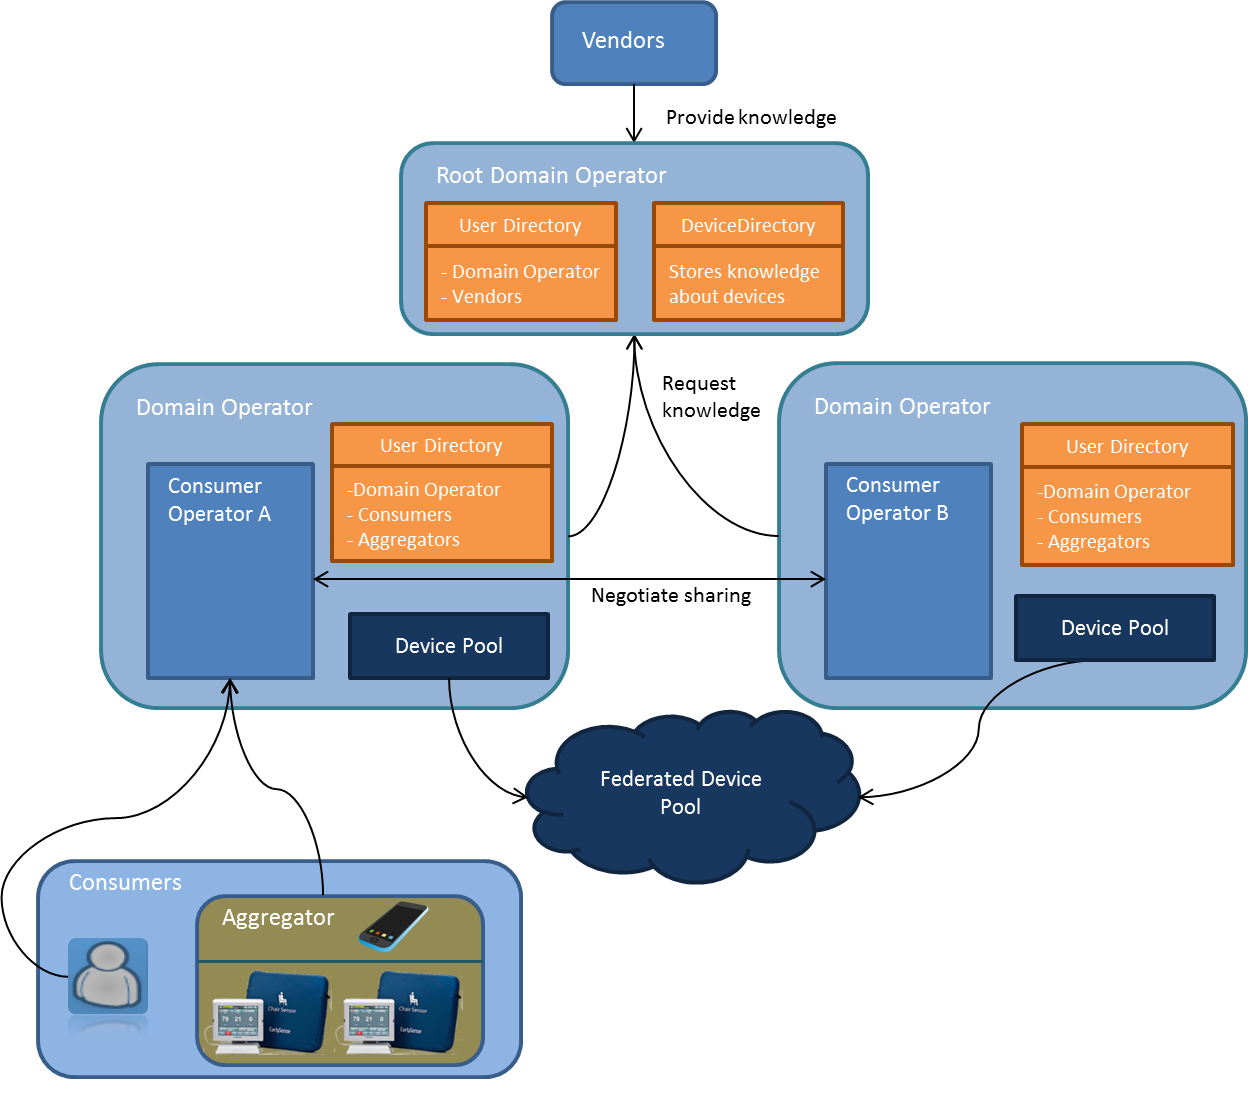
\includegraphics[scale=0.3]{images/design_complete}
	\caption{Detailed Architecture of the Devices Cloud}
	\label{fig:design_complete}
\end{figure}

Every Domain Operator maintain a User Directory and a Device Directory. The earlier is used to authenticate and authorize every entities that can be. The latter is used to store the information about every device operated by the operator.

The Device Directory is particularly important for authorization purposes, because it stores knowledge like the Device Owner and Device Operator for every device. As explained in the Introduction, those two roles are the only ones that are authorized, for example, to revoke a device's access. 

In the framework, the Device Directory could then be compared to the authorization server in the sense that it can map an entity with roles.

This Device Directory has a public interface, the Device Pool, containing the devices they operate. This Device Pool contains only the information that an end customer can see in order to choose which devices he wants to have access to. The different device pools contribute then to a Federated Device Pool, containing all devices available to the customers. Those, when registered to their Domain Operator, can have access to this Federated Pool. Of course, the different pools of devices must be synchronized, but it will not be explained in this thesis.

When a customer has chosen which devices he wants to read the data from, he uses an aggregator, most likely its mobile phone, to integrate the different devices. The authentication of the different actors is first performed (intra Operators, between Customer and Domain Operator, ...), the required data (like drivers) is then retrieved from the Domain Operators or Root Domain Operator and the data can eventually be read from the device.

 \subsection{Entities}
 In \citetitle{reference_thesis}, four main characteristics have been defined for the entities present in the \emph{device cloud}:
 
% \begin{table}[!ht]
% 	\caption{Type of Entities in the Device Cloud}
%	 \centering
	 \def\arraystretch{1.5}
%	 \setlength{\extrarowheight}{15pt}
	 \begin{longtable}{|m{\textwidth}|}
	 	\caption{Type of Entities in the Device Cloud} \\
	 	\hline
	 	\rowcolor{Gray}\textcolor{white}{\textbf{  Entities Characteristics}}
	 	\\ \hline

		
	 	\pbox{\linewidth}{
	 		\vspace*{10pt}
		 	 \textbf{Attachment Entity:} \\
	 		 An attachment refers to any kind of resource usually stored on the file system (e.g.	a picture or a binary). Attachment Entities can have several attachments.
	 		}
	 		\\ \hline
	 	
	 	\pbox{\linewidth}{
	 		\vspace*{10pt}
	 		\textbf{Configurable Entity:} \\
	 		A configurable entity holds a set of configuration entries expressed as key-value pairs. Each entry again is backed by the global entity definition (in the Root Domain). This means, that each local copy of an entity can have two virtual sets of configuration entries.
	 	} \\
 	\hline
 		\pbox{\linewidth}{
 			\vspace*{10pt}
 			\textbf{Location Tagged Entity:} \\
 			An entity whose location can be monitored. This can be an important parameter
 			when having to decide about competing device access re quests or requests to devices
 			that are already provisioned. 
 		} \\
 		\hline
 		\pbox{\linewidth}{
 			\vspace*{10pt}
 			\textbf{Principal Entity:} \\
 			A Principal Entity is an entity that can be authenticated by the User Directory using its EntityID and some kind of security credentials (e.g. certificate or password).
 			Examples are Consumer Operators, Consumers, Aggregators or Vendor. 
 		} \\
 		\hline
 \end{longtable}
 
 in this thesis, the focus will be put on Principal Entities, since it's the most relevant characteristic when designing an authentication framework. However, an entities can have several characteristics at the same time. Every type of entity must then be taken into consideration.
 
 Based on the \emph{device cloud}, a non-exhaustive list of the entities that must maintained the User Directory has been determined:
 
  \def\arraystretch{1.5}
  %	 \setlength{\extrarowheight}{15pt}
  \begin{longtable}{|m{\textwidth}|}
  	\caption{User Directory Entities} \\
  	\hline
  	\rowcolor{Gray}\textcolor{white}{\textbf{  User Directory Entities}}
  	\\ \hline
  	
  	\pbox{\linewidth}{
  		\vspace*{10pt}
  		\textbf{Aggregator:} \\
  		Used for authenticating Aggregators within a Domain.
  	}
  	 \\
  	 Inherit from: Attachment Entity, Configurable Entity, Principal Entity, Location Tagged Entity.
  	\\ \hline
  	\pbox{\linewidth}{
  		\vspace*{10pt}
  		\textbf{Consumer:} \\
		Used for authenticating Consumers within a Domain. 
  	} 
  	\\
  	Inherits from: Attachment Entity, Configurable Entity, Principal Entity, Location Tagged Entity.
  	\\	\hline
  	\pbox{\linewidth}{
  		\vspace*{10pt}
  		\textbf{Consumer Profile:} \\
  		The Consumer Profile is bound to a Consumer and stores preferences or predefined configurations.  
  	} 
  	\\
  	Inherits from: Attachment Entity, Configurable Entity.
  	\\ 	\hline
  	\pbox{\linewidth}{
  		\vspace*{10pt}
  		\textbf{Operators:} \\
  		Used for authenticating Operators within a Domain and store required information, like how to communicate with the Operator. In order to do so, the two following properties have been defined:
  	}
  	\\
  	
  	 \hspace{2em}\hangindent=2em \tabitem \textit{DomainOperator}: flag indicating whether the Operator is a Consumer or a Domain Operator.
  	\\
  	\hspace{2em}\hangindent=2em	\tabitem \textit{ProtocolURI}: defines the endpoint where to contact the Operator (protocol + location), most of the time an absolute URL. 
  	\\
  	Inherits from: Attachment Entity, Configurable Entity, Principal Entity. 
%  	\pbox{\linewidth}{
%  		\vspace*{10pt}
%  		\textbf{Operators:} \\
%  		Used for authenticating Operators within a Domain and store required information, like how to communicate with the Operator. In order to do so, the two following properties have been defined:\\
%  		% 		\begin{itemize}
%  		%  			\item \textit{DomainOperator}: flag indicating whether the Operator is a Consumer or a Domain Operator.
%  		%  			\item \textit{ProtocolURI}: defines the endpoint where to contact the Operator (protocol + location), most of the time an absolute URL. 
%  		%  		\end{itemize}
%  		
%  		Inherits from: Attachment Entity, Configurable Entity, Principal Entity.
%  	} 
  	\\	\hline
  	\pbox{\linewidth}{
  		\vspace*{10pt}
  		\textbf{Vendors:} \\
  		Used for authenticating Vendors within a Domain.
  	} 
  	\\
  	Inherits from: Attachment Entity, Configurable Entity, Principal Entity.
  	\\	\hline
  \end{longtable}
 
In addition to the four entities that must be authenticated, a consumer Profile has been added. this profile is used for storing predefined set of devices that a user needs and the different modules needed for processing the data. To make it clear, let's take the example of a diabetic A who had a brand new sensor installed for measuring the blood glucose level(Google contact lenses, or Apple iWatch for example).

The hospital B is quite familiar with those technologies, but it wishes that the data retrieved can be immediately readable with the CSV format, and not with the proprietary format of Google or Apple. In that case, the hospital can set up a profile where the device (the new sensor) is defined, as well as the module that converts the proprietary format into CSV format.
\linebreak
\linebreak
\linebreak
The reader should now have a good knowledge of the global design and its requirements. The next section introduces him to the authentication and authorization principles and implementations.

\section{Encryption}
Encryption is one of the key principle of network security. It ensures that nobody can have access to protected information even if a message has been intercepted, by encoding the messages. Different algorithms and methods exist, so that only the recipient of a message can decrypt the encoded message.

\subsection{symmetric key}
Some algorithm or protocols are based on a symmetric key. It is assumed that both the sender and the recipient of the messages share a secret (the key). Only the two actors A and B can then encrypt and decrypt the messages thanks to this shared secret key.

Of course, it is assumed that the underlying cryptosystem is strong, so that nobody can decrypt the messages without the key.

This system requires also that the two communicating entities share the secret key from the beginning, which poses the problem of the key distribution. This can be done through physical delivery (A delivers the key to B, or a third party delivers a key to A and B), by using a previous shared key (the new key is sent encrypted with the old key), or by using an encrypted communication with a third party C.
 
\subsection{asymmetric keys}
Other algorithms are based on asymmetric keys. This time, every entity has two keys: a public one $k_{p}$, that can be sent to anybody, and a private $ k_{p}^{-1} $, that is kept secret.

The idea underneath this system is that a message encrypted with $k_{p}$ can only be decrypted with $ k_{p}^{-1} $, and, the other way around, a message encrypted with $ k_{p}^{-1} $ can only be decrypted with $k_{p}$.

Since the public key is accessible to anybody, a asymmetric key based system doesn't show the same key distribution problem.

\subsection{SSL}
SSL is described in \citetitle{freier2011secure}\cite{freier2011secure} as a protocol that "allows client/server applications to communicate in a way that is designed to prevent eavesdropping, tampering, or message forgery".

\section{Authentication}
\subsection{Principles}
\subsection{Based on a symmetric key}
\subsection{Based on asymmetric keys}
\subsection{Based on a One-way function}
Another possibility to authenticate principals is to rely on a so-called One-way function.
\subsubsection{One-Way function}
Such a function $f$ presents the following properties:
\begin{itemize}
	\item \textbf{Easy to compute:} \\
	it can be computed in a polynomial time algorithm.
	\item \textbf{Hard to invert:} \\
	with ($f(x)$), finding $x$ is difficult. In mathematical terms,  for every randomized algorithm $A$ that runs in time polynomial in $n=|x|$, every polynomial $p(n)$, and all sufficiently large $n$: \\
	$ P_{r}[f(A(f(x))) = f(x)] < \dfrac{1}{p(x)}$ 
	\item \textbf{(Optional) collision-free:} \\
	it is unfeasible to find a collision, i.e. $f(x) = f(y)$ and $x \ne y$.
\end{itemize}

As for the symmetric key, it is assumed that the two communicating entities know the One-way function. The advantage of those functions in regards to a symmetric key is that it can be more easily designed than an encryption algorithm, since they don't have to be invertible, but only present the collision-free property. Indeed, for authentication, the collision-free property is particularly important because it is the only way to check the authenticity of a message.

\subsubsection{Proposed prorocol}
\subsection{Shared Authentication Framework}
\subsection{SSO}
\subsubsection{Shibboleth}
\subsubsection{SAML}
\subsection{Kerberos}
\subsection{OpenID and OpenID Connect}


\section{Authorization}
\subsection{Access Control}
\subsubsection{MAC}
\subsubsection{DAC}
\subsubsection{RBAC}
\subsection{In a ditributed environement - OAuth 2.0}



\section{Related work}
Concerning the technology that will be used, several choices are possible. One could rely on a Password-authenticated key agreement \cite{Hao2011}\cite{Pointcheval2012}\cite{Juang2008}, symmetric or asymmetric encryption\cite{Woo1997}\cite{Denning1982}, on the Diameter protocol, the kerberos protocol\cite{Sundareswaran}, the Otway–Rees protocol, openID\cite{Ghazizadeh} and openID connect, SPX\cite{Tardo1991} or some others. A. Liebl tried in 1994 to list the possible authentication protocols, his list is given in appendix 1.